\documentclass[a4paper,11pt]{article}
\usepackage[utf8]{inputenc}
\usepackage{minted}
\usepackage{amsmath}
\usepackage{float}
\usepackage{footmisc}
\usepackage{graphicx}
\usepackage{multirow}
\usepackage[toc,page]{appendix}

\graphicspath{{./figures/}}

\title{\textbf{13. Dijkstra's}}
\author{Kristiāns Vinters}
\date{Fall 2023}

\begin{document}
    \maketitle
    \section*{Introduction}

    I solved the assignment in Go. I used Go because I want to become more familiar with it. Source code and benchmark data is available on GitHub\footnote{https://github.com/Phanty133/id1021/tree/master/13-dijkstra}.

    \section*{Implementation}

    For the implementation, I reused the \texttt{trains} package from the graphs assignment and the \texttt{pqueue} package from the heap assignment. I did not need to make any significant modifications to either package for this assignment. The only modification I made to the \texttt{trains} package is that I added the \texttt{idx} field to the \texttt{City} struct.

    \begin{minted}{go}
type City struct {
    Name      string
    idx       int // Sequential city index set when loading data
    Neighbors []Connection
}
    \end{minted}

    The Dijkstra pathfinding algorithm was implemented as the \texttt{DijkstraFind()} method on the \texttt{NetworkGraph} struct. The implementation of the algorithm is explained with code comments.

    \begin{minted}{go}
func (n *NetworkGraph) DijkstraFind(
    from,
    to string
) (int, []string, error) {
    // Exit early if the from and to cities are the same
    if from == to {
        return 0, []string{from}, nil
    }

    // Get the City objects from the graph by name
    fromCity := n.LookupCity(from)
    toCity := n.LookupCity(to)

    if fromCity == nil {
        return 0, nil, fmt.Errorf("city %s not found", from)
    }

    if toCity == nil {
        return 0, nil, 0, fmt.Errorf("city %s not found", to)
    }

    // Initialize both data structures
    pq := pqueue.NewArrHeap[*PathNode](n.NumCities)
    cityNodes := make([]*PathNode, n.NumCities)

    // Add the starting city to the priority queue, with distance=0
    pq.Add(&PathNode{fromCity, nil, 0, 0}, 0)

    // Iterate until all cities have been visited
    for !pq.Empty() {
        cur, _ := pq.Dequeue()

        // If the current city is the destination, we're done
        if cur.city == toCity {
            // Assemble the path we found and return
            path := make([]string, 0)
            city := cur.city

            for city != nil {
                path = append(path, city.Name)
                city = cityNodes[city.idx].prev
            }

            return cur.dist, path, nil
        }

        // Make sure the current city's Node is counted as visited
        cityNodes[cur.city.idx] = cur

        for _, n := range cur.city.Neighbors {
            node := cityNodes[n.City.idx]

            // If the neighbor city hasn't been visited yet,
            // add it to the queue
            if node == nil {
                node = &PathNode{n.City, cur.city, n.Dist + cur.dist, 0}
                cityNodes[n.City.idx] = node
                pq.Add(node, node.dist)
            }

            // If the neighbor city has been visited,
            // but the current path is shorter,
            // update the neighbor city's Node
            // and update the priority queue
            if node.dist > n.Dist+cur.dist {
                node.dist = n.Dist + cur.dist
                node.prev = cur.city
                pq.Update(node, node.dist)
            }
        }
    }

    return 0, nil, errors.New("no path found")
}
    \end{minted}

    \section*{Benchmarks}

    I benchmarked Dijkstra's algorithm first by searching for the same routes as in the graphs assignment on the \texttt{trains.csv} dataset, and then by searching for routes from Berlin to all other cities in the \texttt{europe.csv} dataset. All searches were performed 100 times, and the median time was used for the results.
    
    \subsection*{Comparison with previous best}

    To compare with the previous best implementation from the graphs assignment, I ran the same routes with Dijkstra's algorithm. The results are shown in Figure \ref{fig:pathfinding}.
    
    \begin{figure}[H]
        \centering
        
        \hspace*{-9.5pt}\begin{tabular}{c|c|c|c|c}
            \textbf{From} & \textbf{To} & \textbf{Dist, min} & \textbf{Previous best, $\mu s$} & \textbf{Dijkstra's, $\mu s$} \\
            \hline
            \hline
            Göteborg & Stockholm & 211 & 58.4 & 2.86 \\
            Göteborg & Umeå & 705 & 28150 & 5.24 \\
            Göteborg & Sundsvall & 515 & 5100 & 4.89   \\
            Malmö & Göteborg & 153 & 61.4 & 1.89 \\
            Malmö & Stockholm & 273 & 31.0 & 2.44 \\
            Malmö & Kiruna & 1162 & 272000 & 5.80 \\
            Stockholm & Sundsvall & 327 & 2770 & 2.86 \\
            Stockholm & Umeå & 517 & 10180 & 4.26 \\
            Sundsvall & Umeå & 190 & 812500 & 1.89 \\
            Umeå & Göteborg & 705 & 108 & 4.26 \\
        \end{tabular}
        \caption{Pathfinding results}
        \label{fig:pathfinding}
    \end{figure}

    The times show that Djikstra's algorithm is significantly faster for all routes, as well as being more consistent. A contributing factor for the reason that the previous best is so inconsistent in its times is that it has to do a linear search over the path visited for every new city it visits, therefore longer routes like the one from Malmö to Kiruna take significantly longer than shorter routes like the one from Malmö to Göteborg.

    \subsection*{Europe graph}

    I benchmarked Dijkstra's algorithm on the \texttt{europe.csv} dataset by searching for routes from Berlin to all other cities. I then plotted the results vs route time, route node count, and number of cities visited during the search. The results are shown in Figures \ref{fig:path-times}, \ref{fig:path-nodes}, and \ref{fig:path-cities} respectively.

    \begin{figure}[H]
        \centering
        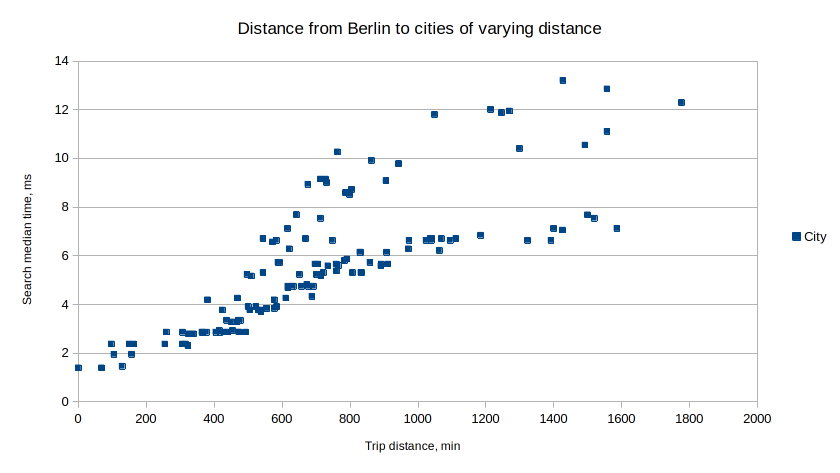
\includegraphics[width=\textwidth]{dists.png}
        \caption{Median lookup time vs route time}
        \label{fig:path-times}
    \end{figure}

    \begin{figure}[H]
        \centering
        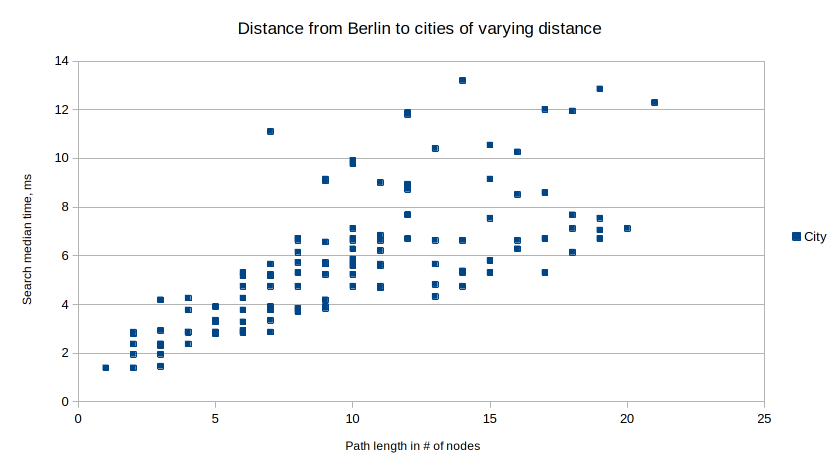
\includegraphics[width=\textwidth]{dists-paths.png}
        \caption{Median lookup time vs route distance in \# of nodes}
        \label{fig:path-nodes}
    \end{figure}

    \begin{figure}[H]
        \centering
        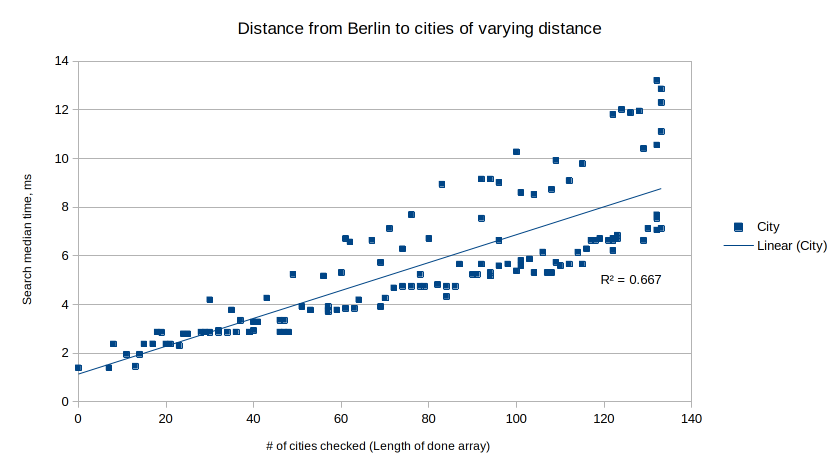
\includegraphics[width=\textwidth]{times-donearr.png}
        \caption{Median lookup time vs \# of nodes visited}
        \label{fig:path-cities}
    \end{figure}

    Figures \ref{fig:path-times} and \ref{fig:path-nodes} show an evident upwards trend in lookup time as route time and route node count increase, however both have a lot of spread in the distribution. Figure \ref{fig:path-cities} shows a clearer, almost linear trend than the other two figures with a tighter spread.
\end{document}
